\question{Динамика относительного движения материальной точки. Переносная и
кориолисова силы инерции. Принцип относительности Галилея. Частные случаи
движения.}

\begin{table}[h!]
\begin{tabular}{C{.4}m{.55\textwidth}}
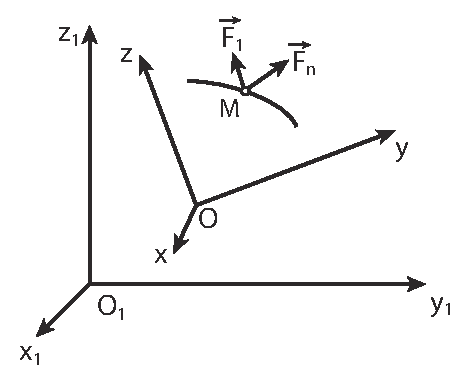
\includegraphics[width=.4\textwidth]{34_01} &
Рассмотрим следующую задачу: имеем две системы отсчета -- неподвижную
\( O_1x_1y_1z_1 \) и подвижную \( Oxyz \). В неподвижной системе отсчета
справедливо основное уравнение динамики: \( m\vec{a} = \sum\vec{F} \), где
\( \vec{F} \) -- равнодействующая всех активных сил.

Выразим абсолютное ускорение через относительное, переносное и кориолисово:

\( \vec{a} = \vec{a}_r + \vec{a}_e +\vec{a}_{cor} \). 
\end{tabular}
\end{table}

Подставляя в основное уравнение динамики, получим:
\[
    m\vec{a}_r = \vec{F} - m\vec{a}_e - m\vec{a}_{cor} = \vec{F} +
    \vec{\varPhi}_e + \vec{\varPhi}_{cor},
\]
где \( \vec{\varPhi}_e = -m\vec{a}_e \) -- переносная сила инерции,
\( \vec{\varPhi}_{cor} = -m\vec{a}_{cor} \) -- кориолисова сила инерции.

Таким образом, основной закон динамики относительного движения материальной
точки выглядит следующим образом:
\[
    m\vec{a}_r = \sum\vec{F} - \vec{\varPhi}_e - \vec{\varPhi}_{cor}.
\]

\subquestion{Частные случаи движения}
\begin{enumerate}
    \item Пусть переносное движение поступательно и равномерно, тогда
    \( \vec{\omega} = 0 \Rightarrow \vec{\varPhi}_{cor} = 0 \),
    \( \vec{a}_e = 0 \Rightarrow \vec{\varPhi}_e = 0 \), а основное уравнение
    динамики примет следующий вид: \( m\vec{a}_r = \sum\vec{F} \).
    
    Отсюда вытекает \emph{принцип относительности Галилея}: не существует таких
    механических опытов, с помощью которых можно определить поступательное и
    равномерное относительное движение.
    
    \item Пусть переносное движение поступательное, но не равномерное:
    \( \vec{\omega} = 0 \Rightarrow \vec{\varPhi}_{cor} = 0 \),
    \( \vec{a}_e \ne 0 \Rightarrow \vec{\varPhi}_e \ne 0 \), тогда:
    \( m\vec{a}_r = \sum\vec{F} + \vec{\varPhi}_e \).
    
    \item Случай относительного покоя: \( \vec{a}_r = 0 \), \( \vec{v}_r = 0 \),
    тогда \( \sum\vec{F} + \vec{\varPhi}_e = 0 \).
\end{enumerate}

\newpage
